\begin{figure}[H]
\centering
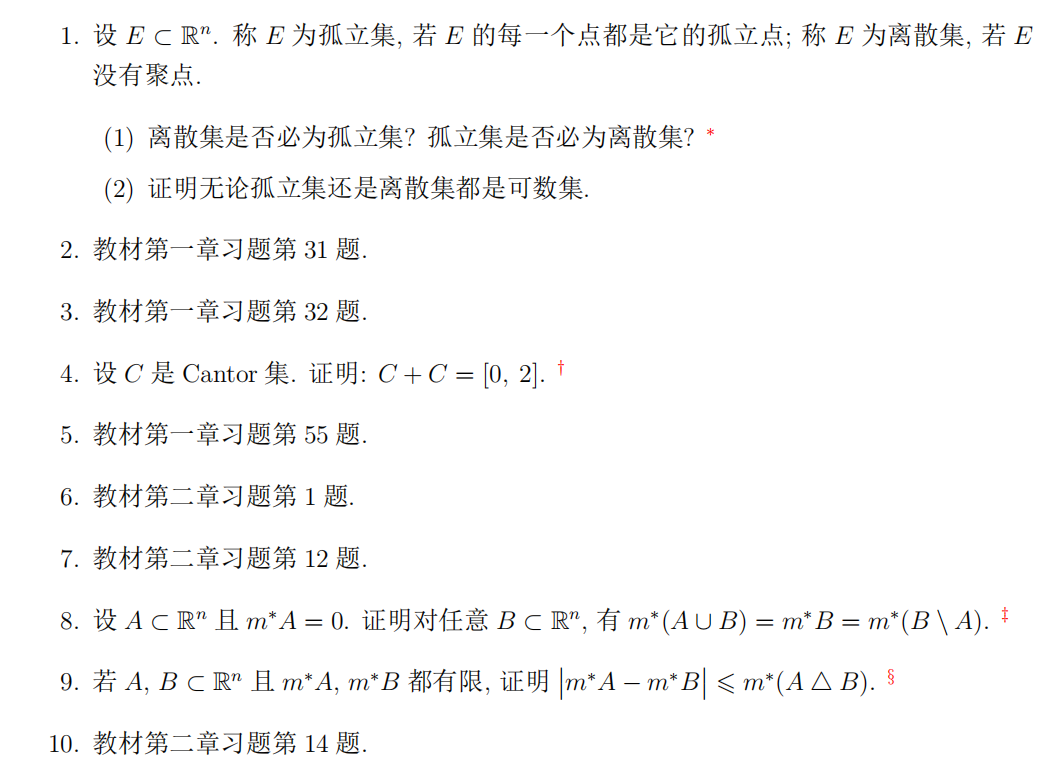
\includegraphics[width=\textwidth]{hw4-2025032809.png}
% \caption{}
\label{}
\end{figure}

\begin{figure}[H]
\centering
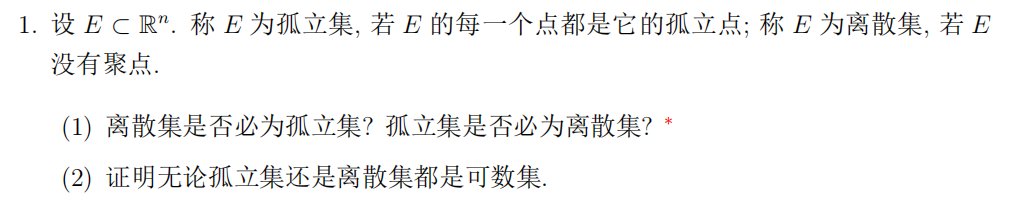
\includegraphics[width=\textwidth]{1-hw4-2025032809.png}
% \caption{}
\label{}
\end{figure}

(1) yes, yes.

(2) $\forall x\in E$, $\exists U_{x}$ s.t.$E\cap U_{x}=\{ x \}$. Since $\mathbb{Q}$ is dense in $\mathbb{R}^{n}$, then $\exists r_{x}\in U_{x}\cap \mathbb{Q}$. Construct
\[
f:E\to \mathbb{Q}\qquad x\mapsto r_{x}
\]
$f$ is clearly one-one, then
\[
\#E=\#f(E)\leq \#\mathbb{Q}=\aleph_0
\]
Thus $E$ is at most countable.

\begin{figure}[H]
\centering
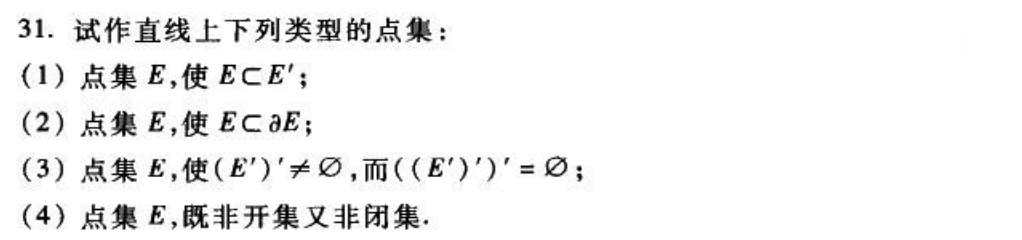
\includegraphics[width=\textwidth]{2-hw4-2025032809.png}
% \caption{}
\label{}
\end{figure}

(1) $(a, b), a, b\in \mathbb{R}$.

(2) $\{ p \}, p\in \mathbb{R}$.

(3) pick $E=\{ 2^{-n}(1+2^{-m}) \}_{m,n=0}^{\infty}$ $m$ then $E'=\{ 2^{-n} \}_{n=0}^{\infty}$, $E''=\{ 0 \}$, $E'''=\varnothing$.

(4) $[a,b)$, $a, b\in \mathbb{R}$.

\begin{figure}[H]
\centering
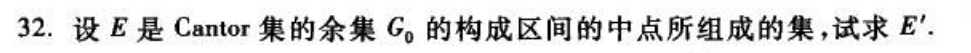
\includegraphics[width=\textwidth]{3-hw4-2025032809.png}
% \caption{}
\label{}
\end{figure}
Claim that $E'=\mathcal{C}$.

First to show that $E\subset \mathcal{C}$. Let
\[
\begin{aligned}
C_0 & =I=[0,1] \\
C_1 & =\left[ 0,\frac{1}{3} \right]\cup\left[ \frac{2}{3},1 \right]  \\
C_2 & =\left[ 0,\frac{1}{9} \right]\cup\left[ \frac{2}{9} ,\frac{1}{3} \right] \cup\left[ \frac{2}{3},\frac{7}{9} \right]\cup\left[ \frac{8}{9},1 \right] \\
 & \dots
\end{aligned}
\]
Denote
\[
\begin{aligned}
M_1 & =\left\{  \frac{1}{2}  \right\} \\
M_2 & =\left\{  \frac{1}{6},\frac{5}{6}  \right\} \\
 & \dots
\end{aligned}
\]
$M_n=\bigcup_{x\in M_{n-1}}\left\{  x\pm\frac{1}{3^{n-1}}  \right\}$. Therefore $E=\bigcup_{n=1}^{\infty}M_n$. Pick $x$ in $E$. It must lie in $M_n$ for some $n$. Then pick the sequence $x,x-\frac{1}{3^{n}},x-\frac{1}{3^{n}}-\frac{1}{3^{n+1}},\dots$, which lies in $E$, with limit point $x-\frac{1}{2\cdot3^{n}}$ which is the nearest point in $\mathcal{C}$. So is $x+\frac{1}{2\cdot3^{n}}$ for the sequence $x,x+\frac{1}{3^{n}},x+\frac{1}{3^{n}}+\frac{1}{3^{n+1}},\dots$. Therefore $\mathcal{C}\subseteq E'$.

If $E'\centernot{\subseteq}\mathcal{C}$, then there is a point $x$ in $E'$ with a sequence $\{ x_1,\dots,x_n,\dots \}$ in $E$ convergent to $x$, but $x\centernot{\in}\mathcal{C}$. Since each $x_n$ is midpoint of $G_0$ then $x_n$ can be any closed to the points in $\mathcal{C}$, as $n\to \infty$. Hence $x\in \mathcal{C}$ which is a contradiction.

\begin{figure}[H]
\centering
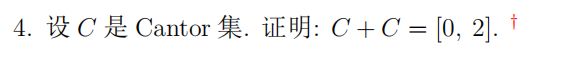
\includegraphics[width=\textwidth]{hw4-2025032810.png}
% \caption{}
\label{}
\end{figure}
Clearly: $C_1+C_1=[0,2]$ and $C_1-C_1=[-1,1]$.

$C_n=\frac{1}{3}C_{n-1}\cup\left( 1-\frac{1}{3}C_{n-1} \right)$, for $n\geq1$. Suppose that $C_{n-1}+C_{n-1}=[0,2]$ and $C_{n-1}-C_{n-1}=[-1,1]$. Then
\[
\begin{aligned}
C_n+C_n & =\left( \frac{1}{3}C_{n-1}\cup\left( 1-\frac{1}{3}C_{n-1} \right) \right)+\left( \frac{1}{3}C_{n-1}\cup\left( 1-\frac{1}{3}C_{n-1} \right) \right) \\
 & =\frac{1}{3}(C_{n-1}+C_{n-1})\cup\left( \frac{1}{3}C_{n-1}+\left( 1-\frac{1}{3}C_{n-1} \right) \right)\cup\left( 2-\frac{1}{3}(C_{n-1}+C_{n-1}) \right)  \\
 & =\frac{1}{3}[0,2]\cup\left( 1+\frac{1}{3}[-1,1] \right)\cup \left( 2-\frac{1}{3}[0,2] \right) \\
 & =\left[ 0,\frac{2}{3} \right]\cup\left[ \frac{2}{3},\frac{4}{3} \right]\cup\left[ \frac{4}{3},2 \right] \\
 & =[0,2]
\end{aligned}
\]
\[
\begin{aligned}
C_n-C_n & =\left( \frac{1}{3}C_{n-1}\cup\left( 1-\frac{1}{3}C_{n-1} \right) \right)-\left( \frac{1}{3}C_{n-1}\cup\left( 1-\frac{1}{3}C_{n-1} \right) \right) \\
 & =\frac{1}{3}(C_{n-1}-C_{n-1})\cup\left( 1-\frac{1}{3}(C_{n-1}+C_{n-1}) \right) \cup\left( \frac{1}{3}(C_{n-1}+C_{n-1})-1 \right) \\
 & =\frac{1}{3}[-1,1]\cup\left[ \frac{1}{3},1 \right]\cup\left[ -1,-\frac{1}{3} \right] \\
 & =[-1,1]
\end{aligned}
\]
By induction, we have
\[
\mathcal{C}+\mathcal{C}=[0,2]
\]
\begin{figure}[H]
\centering
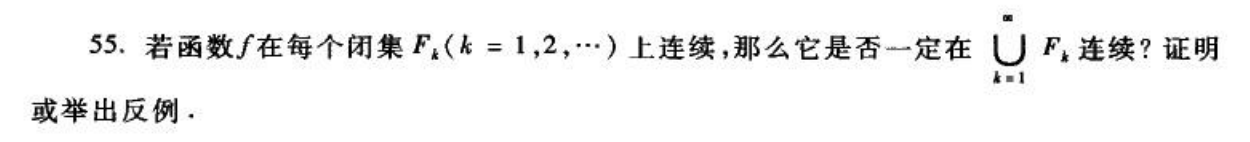
\includegraphics[width=\textwidth]{1-hw4-2025032810.png}
% \caption{}
\label{}
\end{figure}

Counterexample:
\[
f(x)=\begin{cases}
1 & x> 0  \\
0 & x\leq 0
\end{cases}
\]
Pick $F_1=(-\infty,0]$, $F_n=\left[ \frac{1}{n},\infty \right),n\geq2$ then $f$ is constant on each $F_n$, thus continuous. But $f$ is not continuous on $\mathbb{R}=\bigcup_{k=1}^{\infty}F_k$.

\begin{figure}[H]
\centering
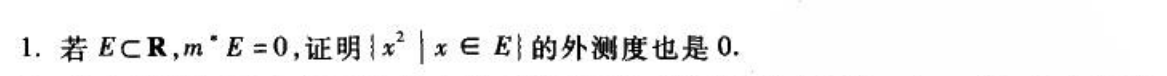
\includegraphics[width=\textwidth]{2-hw4-2025032810.png}
% \caption{}
\label{}
\end{figure}

Denote $E\coloneqq \{ x^2:x\in F \}$, $E_n=E\cap([-n, n]\setminus \{ 0 \}),n\geq1$. Construct a sequence
\[
F_0=F\cap\{ 0 \},F_1=F\cap(0,1],\dots,F_n=F\cap(0,n^2],\dots
\]
Since $m^{*}F=m^{*}\bigcup_{n=0}^{\infty}F_n\leq \sum_{n=0}^{\infty}m^{*}F_n$, it suffices to chech that $m^{*}F_n=0$ for each $n$. Clearly, $m^{*}F_0\leq m^{*}\{ 0 \}=0$. When $n\geq1$,
\[
F_n=F\cap(0,n^2]=\{ x^2: x\in E_n\}
\]
Since $m^{*}E=0$, then $\forall\epsilon>0,\exists \{ I_{n,k} \}_{k=1}^{\infty}$ covering $E_n$ such that
\[
\sum_{k=1}^{\infty} l(I_{n,k})\leq \frac{\epsilon}{2^{n+1}n}
\]
$I_{n,k}\coloneqq(a_{n,k},b_{n,k})$. WLOG $a_{n,k},b_{n,k}$ are positive or negative. Let
\[
J_{n,k}\coloneqq \begin{cases}
(a_{n,k}^2,b_{n,k}^2) & \text{if }a_{n,k}>0 \\
(b_{n,k}^2,a_{n,k}^2) & \text{if }a_{n,k}<0
\end{cases}
\]
Then $\forall x\in E_n$, $x$ must lie in $I_{n,k}$ for some $k$. Then $x^2$ lies in $J_{n,k}$, which means that $\{ J_{n,k} \}_{k=1}^{\infty}$ covers $F_n$, thus
\[
m^{*}F_n\leq \sum_{k=1}^{\infty} l(J_{n,k})=\sum_{k=1}^{\infty} \lvert b^{2}_{n,k}-a_{n,k}^2 \rvert \leq 2n\sum_{k=1}^{\infty} \lvert b_{n,k}-a_{n,k} \rvert =\frac{\epsilon}{2^{n}}
\]
Thus
\[
m^{*}(\{ x^2:x\in E \})=m^{*}\bigcup_{k=1}^{\infty} F_n\leq \sum_{n=1}^{\infty} m^{*}F_n\leq \sum_{n=1}^{\infty} \frac{\epsilon}{2^{n}}=\epsilon
\]
\begin{figure}[H]
\centering
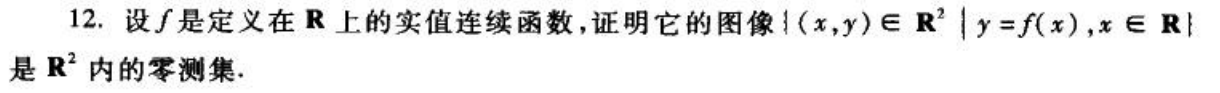
\includegraphics[width=\textwidth]{hw4-2025032812.png}
% \caption{}
\label{}
\end{figure}

Denote that
\[
E_n\coloneqq \{ (x,f(x))\in \mathbb{R}^{2}:x\in[-n,n] \}
\]
Then $f$ is continuous thus uniformly continuous on $[-n-1,n+1]$. For any given $\epsilon>0$, let
\[
A(x)\coloneqq\left\{  y\in(-n-1,n+1):\lvert f(y)-f(x) \rvert<\frac{\epsilon}{4n+4}  \right\}
\]
Then $\{ A(x) \}$ is an open cover of $[-n,n]$. Since $[-n,n]$ is closed and bounded, thus compact. Then there exists $\{ x_1,\dots,x_{r} \}$ such that
\[
[-n,n]\subset \bigcup_{k=1}^{r} A(x_k)
\]
Then
\[
\begin{aligned}
E_n & \subseteq \bigcup_{k=1}^{r} \{ (y,f(y))\in \mathbb{R}^2:y\in A(x_k) \} \\
 & \subseteq \bigcup_{k=1}^{r} (A(x_k)\times (f(x_k)-\epsilon,f(x_k)+\epsilon)) 
\end{aligned}
\]
Then
\[
m^{*}E_n\leq \sum_{k=1}^{r} m^{*}A(x_k)\times m^{*}(f(x_k)-\epsilon,f(x_k+\epsilon))=\frac{\epsilon}{2n+2} \sum_{k=1}^{r} m^{*}A(x_k)\leq \epsilon
\]
Since $\epsilon$ is arbitrary, $m^{*}E_n=0$. Therefore
\[
m^{*}\{ (x,f(x)):x\in \mathbb{R} \}\leq \sum_{n=1}^{\infty} m^{*}E_n=0
\]
\begin{figure}[H]
\centering
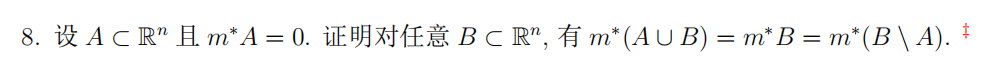
\includegraphics[width=\textwidth]{hw4-2025032819.png}
% \caption{}
\label{}
\end{figure}

It suffices to check that $m^{*}B\leq m^{*}(A\cup B)$. By the definition of outer measure, since $m^{*}A=0$, then $\forall\epsilon>0,\exists \{ P_k \}_{k\geq1}$ covering $A$, s.t.
\[
\sum_{k=1}^{\infty} l(P_k)<\frac{\epsilon}{2}
\]
Pick $\{ I_k \}_{k\geq1}$ covering $B$ s.t.
\[
\sum_{k=1}^{\infty} l(I_k)\leq m^{*}B+\frac{\epsilon}{2}
\]
Put $J_k=I_k\cup P_k$, then $\{ J_k \}_{k=1}^{\infty}$ is a cover of $A\cup B$, then
\[
m^{*}(A\cup B)\leq \sum_{k=1}^{\infty} l(J_k)\leq \sum_{k=1}^{\infty} l(I_k)+\sum_{k=1}^{\infty} l(P_k)\leq m^{*}B+\epsilon
\]
Since $\epsilon$ is arbitrary, thus
\[
m^{*}(A\cup B)\leq m^{*}B
\]
Therefore
\[
m^{*}(A\cup B)=m^{*}B
\]
Since $B=(B\setminus A)\cup A$, then
\[
m^{*}B=m^{*}(B\setminus A)
\]
\begin{figure}[H]
\centering
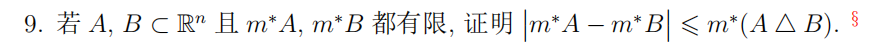
\includegraphics[width=\textwidth]{1-hw4-2025032819.png}
% \caption{}
\label{}
\end{figure}

Since $A\subset(A\setminus B)\cup B$, then
\[
m^{*}A\leq m^{*}(A\setminus B)+m^{*}B
\]
Since $B\subset(B\setminus A)\cup A$ then
\[
m^{*}B\leq m^{*}(B\setminus A)+m^{*}A
\]
Thus
\[
\lvert m^{*}A-m^{*}B \rvert\leq \max\{ m^{*}(A\setminus B),m^{*}(B\setminus A) \}\leq m^{*}(A\setminus B)+m^{*}(B\setminus A)=m^{*}(A\Delta B)
\]
\begin{figure}[H]
\centering
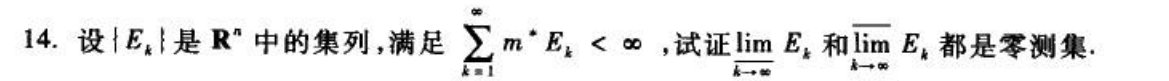
\includegraphics[width=\textwidth]{2-hw4-2025032819.png}
% \caption{}
\label{}
\end{figure}
\[
\varliminf_{ k \to \infty } E_k=\bigcup_{k=1}^{\infty} \bigcap_{n=k}^{\infty} E_n \qquad \varlimsup_{ k \to \infty }E_k= \bigcap_{k=1}^{\infty} \bigcup_{n=k}^{\infty}E_n
\]
NTS: $\varliminf_{ k \to \infty }E_k\subseteq \varlimsup_{ k \to \infty }E_k$. $\forall x\in \bigcup_{k=1}^{\infty}\bigcap_{n=k}^{\infty}E_n$, check that $x\in \bigcap_{k=1}^{\infty}\bigcup_{n=k}^{\infty}E_n$.

NTS: $x\in \bigcup_{n=k}^{\infty}E_n,\forall k\in \mathbb{N}$.

Fix $k'\in \mathbb{N}$, NTS: $x\in \bigcup_{n=k'}^{\infty}E_n$.
\[
x\in \bigcup_{k=1}^{\infty} \bigcap_{n=k}^{\infty} E_n=\left( \bigcup_{k=1}^{k'} \underbrace{ \bigcap_{n=k}^{\infty} E_n }_{ \subseteq E_{k'} } \right)\bigcup \left( \bigcup_{k=k'+1}^{\infty} \underbrace{ \bigcap_{n=k}^{\infty} E_n }_{ \subseteq E_k } \right)\subseteq E_{k'}\cup\left( \bigcup_{k=k'+1}^{\infty} E_k \right)=\bigcup_{k=k'}^{\infty} E_k
\]
Therefore $\varliminf_{ k \to \infty }E_k\subseteq \varlimsup_{ k \to \infty }E_k$.
\[
m^{*}\left( \bigcap_{k=1}^{\infty} \bigcup_{n=k}^{\infty} E_n \right)=\lim_{ k \to \infty } m^{*}\left( \bigcup_{n=k}^{\infty} E_n \right)\leq \lim_{ k \to \infty } \sum_{n=k}^{\infty} m^{*}E_n=0
\]
Hence
\[
m^{*}(\varliminf_{ k \to \infty } E_k)=m^{*}(\varlimsup_{ k \to \infty } E_k)=0
\]